
\documentclass[a4paper,10pt,fleqn, twocolumn]{IEEETran}
\usepackage{amsfonts}
\usepackage{amsthm}
\usepackage{graphicx}
\usepackage{fancyhdr}


\newtheorem{Prop}{Proposition}
\newtheorem{lemma}{Lemma}


\setlength{\parindent}{3em} \setlength{\oddsidemargin}{0in}
\setlength{\textwidth}{6.5in} % sets 1in left and right margins
\setlength{\topmargin}{0.20in} % change to 0.2in for regular latex
%\setlength{\headheight}{0in}
%\setlength{\footheight}{0.5in}
\setlength{\footskip}{0.5in}
\setlength{\textheight}{9.0in} %sets 1in top and bottom margins
\renewcommand{\baselinestretch}{1} %set to 1.5 for double spacing.

\newcommand{\br}{{\mathbf r}}
\newcommand{\bA}{{\mathbf A}}
\newcommand{\ba}{{\bf a}}
\newcommand{\bb}{{\bf b}}
\newcommand{\bc}{{\bf c}}
\newcommand{\bC}{{\bf C}}
\newcommand{\bg}{{\bf g}}
\newcommand{\bG}{{\bf G}}
\newcommand{\bd}{{\bf d}}
\newcommand{\be}{{\bf e}}
\newcommand{\bq}{{\bf q}}
\newcommand{\bs}{{\bf s}}
\newcommand{\bm}{{\bf m}}
\newcommand{\bn}{{\bf n}}
\newcommand{\bu}{{\bf u}}
\newcommand{\bv}{{\bf v}}
\newcommand{\bw}{{\bf w}}
\newcommand{\bx}{{\bf x}}
\newcommand{\by}{{\bf y}}
\newcommand{\bz}{{\bf z}}
\newcommand{\bbf}{{\bf f}}
\newcommand{\bE}{{\bf E}}
\newcommand{\bF}{{\bf F}}
\newcommand{\bL}{{\bf L}}
\newcommand{\bM}{{\bf M}}
\newcommand{\bN}{{\bf N}}
\newcommand{\bS}{{\bf S}}
\newcommand{\bT}{{\bf T}}
\newcommand{\bD}{{\bf D}}
\newcommand{\bX}{{\bf X}}
\newcommand{\bP}{{\bf P}}
\newcommand{\bQ}{{\bf Q}}
\newcommand{\bI}{{\bf I}}
\newcommand{\bR}{{\bf R}}
\newcommand{\bU}{{\bf U}}
\newcommand{\bV}{{\bf V}}
\newcommand{\bW}{{\bf W}}
\newcommand{\bY}{{\bf Y}}
\newcommand{\bZ}{{\bf Z}}
\newcommand{\bJ}{{\bf J}}
\newcommand{\bB}{{\bf B}}
\newcommand{\bzero}{{\bf 0}}
\newcommand{\bgamma}{{\mbox {\boldmath $\gamma$}}}
\newcommand{\btheta}{{\mbox {\boldmath $\theta$}}}
\newcommand{\bLambda}{{\mbox {\boldmath $\Lambda$}}}
\newcommand{\bPsi}{{\mbox {\boldmath $\Psi$}}}
\newcommand{\bPhi}{{\mbox {\boldmath $\Phi$}}}
\newcommand{\bcA}{{\mbox {\boldmath ${\cal A}$}}}
\newcommand{\bcB}{{\mbox {\boldmath ${\cal B}$}}}
\newcommand{\bcC}{{\mbox {\boldmath ${\cal C}$}}}
\newcommand{\bcD}{{\mbox {\boldmath ${\cal D}$}}}
\newcommand{\bcF}{{\mbox {\boldmath ${\cal F}$}}}
\newcommand{\bcN}{{\mbox {\boldmath ${\cal N}$}}}
\newcommand{\bcR}{{\mbox {\boldmath ${\cal R}$}}}
\newcommand{\bcS}{{\mbox {\boldmath ${\cal S}$}}}
\newcommand{\bcH}{{\mbox {\boldmath ${\cal H}$}}}
\newcommand{\bcI}{{\mbox {\boldmath ${\cal I}$}}}


\title{Blind Adaptive Decision Feedback Interference Cancellation}
\author{Shu Wang, Sang G. Kim, Li-H. Sun, Hobin Kim, Suk W. Lee and Byung K. Yi\\ LGE Mobile Research (LGEMR),\\ San Diego, CA 92131}
\date{}
\begin{document}
\maketitle
\begin{abstract}\small
Interference cancellation is one of the multiuser detection
strategies for suppressing interference effects and consequently
improving system performance. In this paper, a blind decision
feedback interference cancellation framework, as well as several
implementations using least squares, maximum likelihood and
minimum mean squared error criteria, are proposed for solving the
CDMA near-far problem. Compared with existing blind detectors, the
proposed framework requires a minimum number of previously
received signals and no subspace separation or sequence estimation
operation. The computation complexity and detection delay can
therefore be much reduced. Theoretical analysis and computer
simulations are provided to demonstrate the performance of the
proposed schemes.
\end{abstract}
\section{Introduction}
Interference cancellation (IC) is the strategy for forming an
estimate of various interference, including intersymbol
interference (ISI), co-channel interference (CCI), adjacent
channel interference (ACI), etc., and subtracting it from received
signals before detection. Compared with other detection
strategies, interference cancellation focuses more on interference
estimation and different interference estimation methods may lead
to different interference cancellation
schemes~\cite{Verd98,Wang02b} such as successive
cancellation~\cite{Kohno91}, multistage detection~\cite{Vara88},
decision-feedback interference
cancellation~\cite{Kave85,Duel93,Duel95}, etc. Decision-feedback
interference cancellation (DFIC), including minimum mean squared
error (MMSE) decision-feedback detection~\cite{Kave85} and
decorrelating decision-feedback detection~\cite{Duel93,Duel95}, is
the decision-driven detection scheme that combines several
features of successive interference cancellation and multistage
detection~\cite{Verd98}. Recent research has been devoted to
semiblind/blind implementation of interference cancellation as
well as other multiuser
detectors~\cite{Madh94,Madh98,Wang98,Zhang02} for the practical
applications where only desired users's information is available.
For most semiblind/blind implementations, many adaptive filter
techniques, e.g., Wiener filtering~\cite{Madh94}, Kalman
filtering~\cite{Zhang02} and subspace~\cite{Wang98} techniques,
are among the most popular approaches. However, these approaches
are known to be too complicated or slow for many dynamic high-data
rate situations.

Decision-feedback techniques have been intensively discussed for
channel equalization. In single-user decision-feedback
equalization, previous decision outputs are feeded back for
eliminating ISI and detecting the current symbol. It is known to
have the complexity close to linear equalization while its
performance is close to maximum likelihood equalization. Similarly
in multiuser DFIC, previous decision outputs as well as other
users' decision outputs are utilized for helping detect desired
users's current information~\cite{Madh94,Madh98,Wang98,Verd98}. In
conventional DFIC~\cite{Verd98}, it is shown that other user's
current decision outputs are enough for detecting desired
information providing all users' signal signatures are known. In
blind implementations of DFIC as well as other ICs, previous
received signals and decision outputs are reused to separate
signal subspaces or adapt filters for interference
estimation~\cite{Madh98,Wang98}. The problem with existing DFIC
approaches is that either subspace separation or filter adapt
procedure isn't trivial and may not be fast enough for many
fast-fading channels.

In order to solve the near-far problem with minimum prior
knowledge and computation complexity~\cite{Wang03d,Wang05A}, we
provide an alternative blind DFIC framework, which requires a
small amount of previously received signals for estimating
interference and detecting desired signals. Different to existing
approaches, a minimum number of previously received symbols are
required in addition to desired user(s)' signatures and timing. No
other users' signal signatures or signal subspaces separation is
necessary here. Hence both the complexity and detection delay are
much reduced. This makes it an attractive candidate for
interference cancellation in high data rate systems. Theoretical
analysis and computer simulations are finally presented to
demonstrate the performance of these blind detectors. The proposed
framework and approaches can be easily applied for asynchronous
CDMA.
\section{System Model And Problem Description}
We consider forward-link transmissions in a single-cell DS/CDMA
system. There are $K$ active users over the multipath channel with
$P$ strong paths~\footnote{Strong paths are those to be explicitly
combined by RAKE receiver.} and the channel is an additive white
Gaussian noise (AWGN) channel. The baseband representation of the
received signal due to user $k$ is given by

\begin{equation}
\begin{array}{rcl}
r_k(t)&=&\sum\limits_{p=1}^{P}\alpha_{pk}A_k[n]
b_k[n]c_k(t-nT-\tau_p)
\end{array}
\end{equation}
\noindent where $\alpha_{pk}$ is the $p$th path loss of user $k$'s
signal, $b_k{[n]}$ is the $n$th bit sent by user $k$. We assume
that the $\left\{b_k{[n]}\right\}$ are independent and identically
distributed random variables with $E\left\{b_k{[i]}\right\}=0$ and
$E\left\{|b_k{[i]}|^2\right\}=1$. The parameters $c_k(t)$ denote
the normalized spreading signal waveform of user $k$ during the
interval $[0,\ T]$, $\tau_1\leq\tau_2\leq\ldots\leq\tau_P$,
denotes $P$ different transmission delays from the base station to
user $k$ and $A_k[n]$ is the amplitude of the received signal for
user $k$ at time $t=n$. The total baseband signal received by user
$k$ is
\begin{equation}
\begin{array}{rcl}
\tilde{r}(t)&=&\sum\limits_{k=1}^{K}r_k(t)
\end{array}
\end{equation}
The received signal $\tilde{r}(t)$ is passed through the
corresponding chip matched filter (CMF) $\phi(t)$ and RAKE
combiner. The combined output $r(t)$ is~\footnote{Without loss of
the generality, we drop the time index $n$ in the following
discussion.}
\begin{equation}\hspace{-0.0in}
\begin{array}{rcl}
r(t)&=&A_k b_k c_k(t-nT-\tau_1)\otimes \phi(t-\tau_1)+ \\
&&\hspace{0.0in} m_{\rm ISI}(t) + m_{\rm MAI}(t) + n(t)
\end{array}\label{r_t}
\end{equation}
\noindent where
\begin{equation} \hspace{-0.05in}
\begin{array}{rcl}
 m_{\rm ISI}(t)&=&\\
 &&\hspace{-0.83in}\sum\limits^{P}_{p\neq
q}\beta_{qk} \alpha_{pk}A_kb_kc_k(t-nT+\tau_{q1}-\tau_1)\otimes
\phi(t-\tau_1)
\end{array}
\end{equation}
\noindent is the ISI to user $k$,
\begin{equation} \hspace{-0.17in}
\begin{array}{rcl}
m_{\rm MAI}(t)&=&\sum\limits_{i\neq
 k}^{K}A_ib_ic_i(t-nT-\tau_1)\otimes\phi(t-\tau_1)+\\
 &&\hspace{-0.75in}\sum\limits_{i\neq
 k}^{K}\sum\limits^{P}_{p\neq
q}\beta_{qk}
\alpha_{pi}A_ib_ic_i(t-nT+\tau_{q1}-\tau_p)\otimes\phi(t-\tau_1)
\end{array}
\end{equation}
\noindent is the MAI to user $k$, $\beta_{qk}$ is the weight of
the $q$th RAKE finger with
$\sum\limits_{q=1}^{P}\beta_{qk}\alpha_{qk}=1$ and $\tau_{q1} =
\tau_{q}-\tau_1$ is the propagation delay difference between the
$1$st path and $p$th path. $\otimes$ denotes the convolutional
product. $n(t)$ is AWGN with variance $\sigma^2$. The user $k$'s
RAKE output can be sampled at $f_s=1/T_s$ and straightforwardly
expressed by
\begin{equation}\hspace{-0.1in}
\begin{array}{rcl}
\br&=&\left[
\matrix{r(nT+T_s+\tau_1)&\ldots&r(nT+LT_s+\tau_1)}\right]^{\rm
T}\\
 &=&\sum\limits_{k=1}^{K} A_k b_k \bs_k + \bn \\
 &=&\bS \bA \bb + \bn
\end{array}\label{r_sync}
\end{equation}
\noindent where $\bS=[\bs_1\ \bs_2\ \ldots\ \bs_K]$ is the
received spreading sequence matrix combined with both ISI and MAI
information, and $L=T/T_s$ is the number of samples per symbol,
which usually is not less than the spreading gain $L_c$. Because
of $m_{\rm MAI}(t)$ existing in the received signal $r(t)$, the
performance of conventional matched filter receiver suffers from
the so-called near-far problem~\cite{Verd98} and interference
cancellation is one of the receiver techniques for solving this
problem.

\section{Blind Interference Cancellation}

Without loss of the generality, the signals for the first $G$
desired users will be detected here with
$\bS_1=\left[\matrix{\bs_1&\bs_2&\ldots&\bs_G}\right]$ known
beforehand. Before this, we assemble $M$ previously received and
detected signal vectors into
\begin{equation}
\begin{array}{rcl}
\bcS&=&\bigl[\matrix{{\br}[n-1]&{\br}[n-2]&\ldots&{\br}[n-M]}\bigr]\\
&=&\bS\bA\bB+\bN\\
&=&\bS_1\bA_1\bB_1+\bS_2\bA_2\bB_2+\bN
\end{array} \label{bcs}
\end{equation}
\noindent where $\bB=\bigl[\bB_1^{\rm H}\ \bB_2^{\rm H}\bigr]^{\rm
H}$ is the data matrix for $\bcS$, $\bS_2$ is the original
interfering signals' signatures, $\bA_1$, $\bA_2$, $\bB_1$ and
$\bB_2$ are the amplitude matrices and data matrices for desired
users and interfering users, respectively. Obviously The minimum
number of received signals a receiver requires for possibly
distinguishing all $K-G$ interfering users is $M=K-G$ and the rank
of $\bB_2$ is $\bcR\left(\bB_2\right)=K-G$ at this time. With
(\ref{bcs}), the interference subspace can be approximated by
$\bar\mathbb{S}_{1}=\mbox{span}\left\{\bs_m | m=G+1,\ \ldots\
K\right\}\approx\mbox{span}\left\{\bcS-\bS_1\bA_1\bB_1\right\}$
providing the signal-to-noise ratio (SNR) is high enough. And the
MAI $\bm$ can be rewritten by
\begin{equation}\hspace{-0.0in}
\begin{array}{rcl}
\bm &=&\bS_2\bA_2\bb_2\\
&=&\bigl(\bcS-\bS_1\bA_1\bB_1-\bN\bigr)\bB_2^{+}\bb_2\\
&=&\bcS\bbf-\bS_1\bD_1\bbf+\tilde{\bn}
\end{array}\label{bm}
\end{equation}
\noindent where $\bbf=\bB_2^{+}\bb_2$ denotes a projection of
$\bm$ onto the interfering subspace of $\bS_2\bA_2\bB_2$,
$\bD_1=\bA_1\bB_1$ and $\tilde{\bn}=-\bN\bB_2^{+}\bb_2$.

With (\ref{bm}), it shows that $\bm$ can be estimated providing
$\bbf$ is known. In order to estimate $\bbf$, we perform
QR-decomposition on $\bS_1$ so that~\cite{Huff91,Verd98}
\begin{equation}
\begin{array}{rcccl}
\bS_1&=&\bQ_1\bR_1&=&\bQ_{11}\bR_{11}
\end{array},
\end{equation}
\noindent where $\bQ_1=\left[\bQ_{11}\
\bQ_{12}\right]\in\mathbb{R}^{L\times L}$ is orthogonal and
$\bR_1=[\bR_{11}^{\rm H}\ \bzero^{\rm H}]^{\rm
H}\in\mathbb{R}^{L\times G}$, and apply $\bQ_{12}^{\rm H}$ on
(\ref{bm}) to get
\begin{equation}
\begin{array}{rcl}
\bQ_{12}^{\rm H}\bm&=&\bQ_{12}^{\rm H}\bcS\bbf+\bQ_{12}^{\rm
H}\tilde\bn
\end{array}.
\end{equation}
\noindent Since
\begin{equation}\hspace{-0.0in}
\begin{array}{rcl}
\bQ_{12}^{\rm H}\br&=&\bQ_{12}^{\rm H}\bm + \bQ_{12}^{\rm H}\bn
\end{array},
\end{equation}
\noindent $\bbf$ can be estimated from
\begin{equation}\hspace{-0.0in}
\begin{array}{rcl}
\bQ_{12}^{\rm H}\br&=&\bQ_{12}^{\rm H}\bcS\bbf+\bQ_{12}^{\rm
H}\bar\bn
\end{array},\label{f2}
\end{equation}
\noindent where $\bar\bn=\tilde\bn+\bn$.

After $\bbf$ is estimated, $\bm$ can be estimated using (\ref{bm})
and extracted from $\br$ so that the desired information vector
$\bb_1$ as well as $\bA_1$ can be detected and estimated from
\begin{equation}
\begin{array}{rcl}
\bS_1\bd_1&\approx&\br-\left(\bcS-\bS_1\hat\bD_1\right)\hat{\bbf}
\end{array},\label{br_bm}
\end{equation}
\noindent where $\bd_1=\bA_1\bb_1$, $\hat\bD_1$ denotes previous
detection outputs from $\bcS$ and $\hat{\bbf}$ denotes an estimate
of $\bbf$. This can be done using either Viterbi algorithm or
other sub-optimal detection schemes. This can be shown in Fig. 1.
Since the previous decision outputs $\hat\bD_1$ are used for
estimating $\bm$ and $\bA_1$ and detecting $\bb_1$, this framework
is named blind decision-feedback interference cancellation. Though
this framework is presented as a two-stage approach here, it can
be implemented in a joint detection fashion with simultaneously
estimating $\bd_1$ and $\bbf$.

\begin{figure} \center{
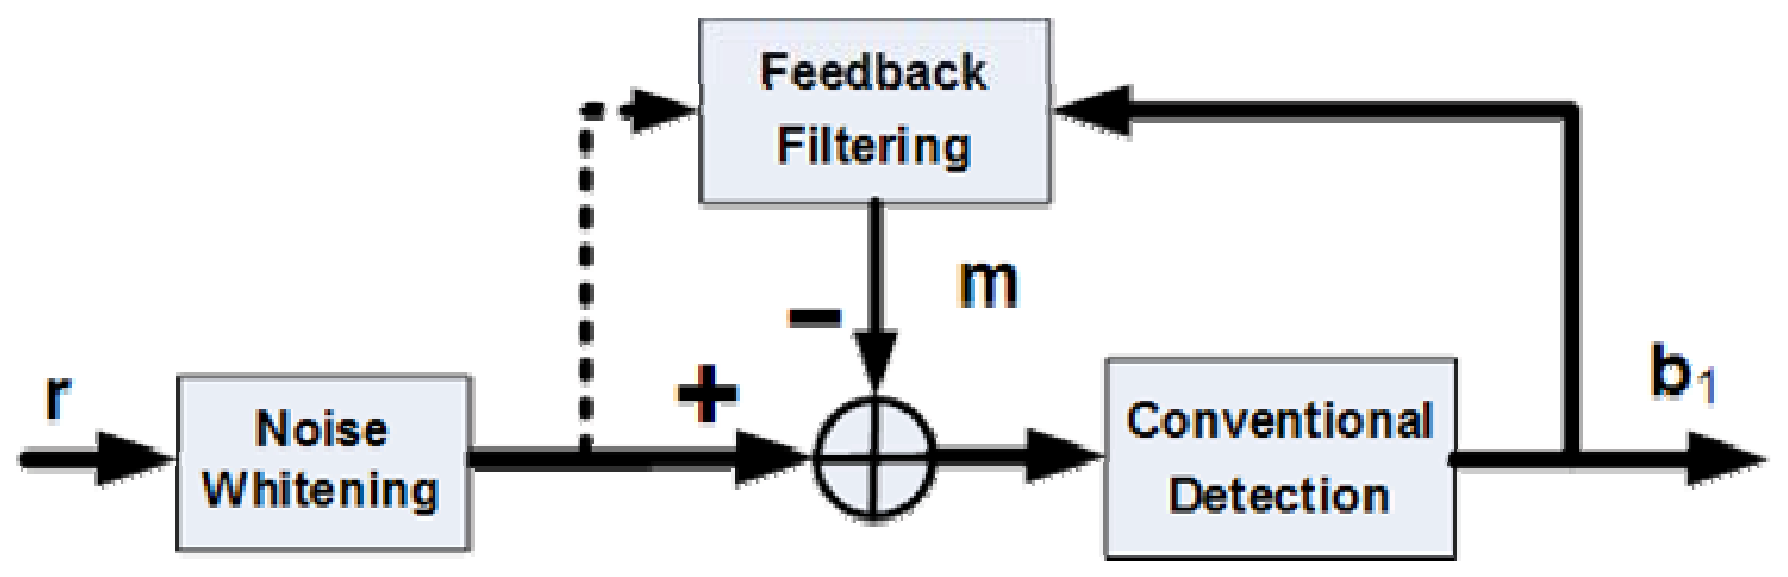
\includegraphics[width=3.2in]{BDFIC1.eps}
\caption{A group-wised decision feedback interference cancellation
block diagram} }\label{DFIC}
\end{figure}

\subsection{\em Least Squares Interference Cancellation}
In classic least squares estimations, the observation matrix is
assume to be error-free so that all estimation errors are supposed
to come from $\br$. This can be expressed by~\cite{Huff91}
\begin{equation}\hspace{-0.09in}
\begin{array}{l}
\left[\matrix{{\hat\bd}_{1\rm LS}\cr\bbf_{\rm
LS}}\right]=\mbox{arg}\min\limits_{\bx}\left\|\br-\bG\bx\right\|_2
\end{array}\label{b_LS}
\end{equation}
\noindent where
\begin{equation}
\begin{array}{rcl}
\bG&=\left[\matrix{\bS_1&\left(\bcS-\bS_1\bD_1\right)}\right]
\end{array}.
\end{equation}
\noindent Therefore the desired vector $\bd_1$ can be estimated by
\begin{equation}\hspace{-0.0in}
\begin{array}{rcl}
\left[\matrix{{\hat\bd}_{1\rm LS}\cr\bbf_{\rm
LS}}\right]&=&\bG^{+}\br.
\end{array}\label{b_LS_IC}
\end{equation}
\noindent where $\left[\cdot\right]^{+}$ denotes the general
inverse operation.

\subsection{\em Mixed Least Squares Interference Cancellation}
In (\ref{b_LS}), it assumes that there exist errors or noises on
both $\bS_1$ and $\left(\bcS-\bS_1\bD_1\right)$. Obviously this is
not true since $\bS_1$ is known to be noise-free. To maximize the
accuracy of estimating $\bd_1$, it is natural to require $\bS_1$
to be unperturbed while keep $\bS_2$ estimated. For this, $\br$
can be re-written as
\begin{equation}
\begin{array}{rcl}
\br&=&\bS_1\left(\bd_1+\bD_1\hat\bbf\right)-\bcS\hat{\bbf}+\bar\bn
\end{array}.\label{br_bm2}
\end{equation}
The mixed least squares (MLS) interference cancellation can be
written by
\begin{equation}\hspace{-0.07in}
\begin{array}{l}
\left[\matrix{\hat{\bS}\cr\left[\matrix{\hat{\bd}_{1}+\bD_{1}\hat\bbf\cr\hat\bbf}\right]_{\rm
MLS}}\right]=\mbox{arg}\min\limits_{\bZ\
\by}\left\|\left[\matrix{\bcS\cr\br}\right]-\left[\matrix{\bZ\cr\left[\bS_1\
\bZ\right]\by}\right]\right\|_2
\end{array}.
\end{equation}
\noindent If $\sigma_{K-G}'>\sigma_{K-G+1}$, the MLS estimation of
$\bbf$ is~\cite{Huff91}
\begin{equation}\hspace{-0.070in}
\begin{array}{l}
{\bbf_{\rm MLS}}=\left(\bcS^{\rm H}\bQ_{12}\bQ_{12}^{\rm
H}\bcS-\sigma_{K-G+1}^{2}\bI\right)^{-1}\bcS^{\rm
H}\bQ_{12}\bQ_{12}^{\rm H}\br
\end{array}\label{f_MLS}
\end{equation}
\noindent where $\sigma_{K-G}'$ and $\sigma_{K-G+1}$ are the
$(K-G)$th and $(K-G+1)$th largest singular value of $\bQ_{12}^{\rm
H}\bcS$ and $\bQ_{12}^{\rm H}\left[\matrix{\br&\bcS}\right]$. The
MLS-IC $\hat{\bd}_{1\rm MLS}$ can be expressed by
\begin{equation}\hspace{0.0in}
\begin{array}{rcl}
\hat{\bd}_{1\rm
MLS}&=&\bS_{1}^{+}\br-\bS_{1}^{+}\left({\bcS}-{\bS}_{1}{\bD_1}\right){\bbf_{\rm
MLS}}
\end{array}\label{b_MLS_IC}
\end{equation}

\subsection{\em Maximum Likelihood Interference Cancellation}
In maximum likelihood interference cancellation (ML-IC), $\bd_1$
is estimated with maximizing the probability density function
(PDF) $p(\br;\ \bd_{1},\ \bbf)$. It is known that ML estimator
asymptotically is the minimum variance unbiased (MVU) estimator
though it is not optimal in general. For the linear Gaussian
signal model in (\ref{br_bm}), ML-IC can be written by
\begin{equation}\hspace{-0.12in}
\begin{array}{rcl}
\left[\matrix{{\hat\bd}_{1\rm ML}\cr\bbf_{\rm
ML}}\right]&=&\mbox{arg}\min\limits_{\bx}\left\{\mathbf\delta^{\rm
H}\bR_{\bar\bn}\mathbf\delta\right\}
\end{array}
\end{equation}
\noindent where the estimation error vector
\begin{equation}
\begin{array}{rcl}
\mathbf\delta&=&\br-\bG\bx
\end{array}.
\end{equation}
Therefore the ML estimation of $\bd_1$ can be given by
\begin{equation}
\begin{array}{rcl}
\left[\matrix{{\hat\bd}_{1\rm ML}\cr\bbf_{\rm
ML}}\right]&=&\left(\bG^{\rm
H}\bR_{\bar\bn}\bG\right)^{-1}\bG^{\rm H}\bR_{\bar\bn}^{-1}\br
\end{array}.\label{b_ML_IC}
\end{equation}

\subsection{\em Mini. Mean-Square Error Interference Cancellation}
With MMSE criterion, $\bd_{1}$ is estimated with minimizing the
Bayesian mean squared error (BMSE):
\begin{equation}\hspace{-0.0in}
\begin{array}{rcl}
\be_{\rm
BMSE}&=&\mbox{E}\left\|\left[\matrix{\hat\bd_{1}\cr\hat\bbf}\right]-\left[\matrix{\bd_{1}\cr\bbf}\right]\right\|_2^2
\end{array}.
\end{equation}
\noindent The MMSE estimation can then be written by
\begin{equation}\hspace{-0.15in}
\begin{array}{l}
\left[\matrix{{\hat\bd}_{1\rm MMSE}\cr\bbf_{\rm
MMSE}}\right]=\mbox{arg}\min\limits_{\bx}\mbox{E}\left\|\br-\bG\bx\right\|_2
\end{array}\label{MMSE_IC}
\end{equation}
\noindent and, if $\br$, $\bd_{1}$ and $\bbf$ are jointly
Gaussian, it can be solved by
\begin{equation}
\begin{array}{rcl}
\left[\matrix{{\hat\bd}_{1\rm MMSE}\cr\bbf_{\rm
MMSE}}\right]&=&\left(\bR_{\bx}+\bG^{\rm
H}\bR_{\bar\bn}\bG\right)^{-1}\bG^{\rm H}\bR_{\bar\bn}^{-1}\br
\end{array}\label{b_MMSE_IC}
\end{equation}
\noindent where
\begin{equation}
\begin{array}{rcl}
\bR_{\bx}&=&\mbox{E}\left\{\left[\matrix{\bd_{1}\bd_{1}^{\rm
H}&\bd_{1}\bbf^{\rm H} \cr \bbf\bd_{1}^{\rm H}&\bbf\bbf^{\rm
H}}\right]\right\}
\end{array}.%\label{b_ML_IC}
\end{equation}
\section{Implementation Issues}
\subsection{Adaptive Detection}

\subsection{Iterative Detection}


\section{Performance Analysis}
\subsection{\em Geometric Explanation}
It is known that conventional decorrelating detection can be
interpolated as an oblique projection of received signals onto
desired users' signal subspace
$\mathbb{S}_{1}=\mbox{span}\left\{\bs_g | g=1,\ 2,\ \ldots ,\
G\right\}$ along its complementary interference subspace
$\bar\mathbb{S}_{1}$~\cite{Elda02} while MMSE detection can be
taken as a balance between single-user matched filter and
decorrelating detector with the same asymptotic multiuser
efficiency (AME) and near-far resistance (NFR) as decorrelating
detection. In the proposed least-squared DFIC, each received
signal is orthogonally projected onto the signal subspace
$\mathbb{S}_{1}^{\perp}=\mbox{span}\left\{\left(\bQ_{12}\bQ_{12}^{\rm
H}\right)\bs_m | m=G+1,\ \ldots\ K\right\}$, which is orthogonal
complementary to $\mathbb{S}_{1}$ for interference estimation.

\subsection{\em Comparison with Existing Blind Detectors}
The comparison between the proposed framework and other major
schemes is presented in Table~1. The proposed framework only
requires $M$, where $L\ge M\ge (K-G)$, previous received signal
for signal detection and its complexity is closed to conventional
detectors while other blind approaches typically requires a lots
more than $L$ signals~\cite{Madh94,Wang98,Zhang02}.
\begin{figure*}[t]\label{SchemComp}
\center{Table 1. The comparison of the proposed framework and
other detection approaches}
\begin{center}
\begin{tabular}{lcccc}
Parameters & Conv. DF-IC & Blind MMSE & Subspace Approaches & Blind DF-IC\\
\hline
\hline
Signature of desired user(s) & $\mathbf\surd$ & $\mathbf\surd$ &  $\mathbf\surd$ & $\mathbf\surd$ \\
Signature of other users & $\mathbf\surd$ & &  \\
Timing of desired user(s)  & $\mathbf\surd$ & $\mathbf\surd$ & $\mathbf\surd$ & $\mathbf\surd$ \\
Timing of other users  & $\mathbf\surd$ & & & \\
Received amplitudes  & $\mathbf\surd$ & &  &\\
ECC decoding-integratable& $\mathbf\surd$ &&& $\mathbf\surd$ \\
Initialization~{\small *} &  & $\ge L$ & $\ge L$ & $M$\\
Latency & $K$ & $1$ & $1$ & $1$ \\
Complexity order & $K$ & $1$ & $1$ & $1$ \\
\hline \hline \multicolumn{5}{l}{\small * For blind MMSE or
subspace-based approaches, it typically requires many more than
$L$ signals for initialization.}
\end{tabular}
\end{center}
\end{figure*}

\subsection{\em AME and Near-Far Resistance}
A commonly used performance measure for a multiuser detector is
AME and NFR~\cite{Verd98}. Since the proposed algorithms converges
to the conventional decorrelating detector as $\sigma^2\rightarrow
0$, their AME and near-far resistance are identical to the
decorrelating detector:
\begin{equation}
\begin{array}{rcl}
\bar{\eta}_k&=&\frac{1}{\left[\bR^{+}\right]_{kk}}
\end{array}.
\end{equation}

\subsection{\em On the new noise vector $\bar\bn$}
Though it is easy to verify that
$\mbox{E}\left\{\bar\bn\right\}=\bzero$, the covariance matrix of
$\bar\bn$ is not easy to be decided because of the unknown PDF of
$\bB_2^{+}$. Following Girko's law, providing $\alpha=(K-G)/M$ is
fixed, the diagonal element of
$\frac{1}{M}\left(\bB_2^{+}\bb_2\right)\left(\bB_2^{+}\bb_2\right)^{\rm
H}$ can be approximated to be $1-\alpha$ with $K$, $M$
$\rightarrow\infty$~\cite{Muller}. And the covariance matrix of
$\bar\bn$ can be expressed by
\begin{equation}
\begin{array}{rcl}
\bR_{\bar\bn}&=&\frac{2M+K-G}{M}\sigma^{2}\bI
\end{array}.\label{noise_var_new}
\end{equation}

\subsection{\em CRLB for $\bd_1$ and $\bbf$ Estimation}
The Cram\'{e}r-Rao Lower Bound (CRLB) is given by the inverse of
the Fisher information matrix (FIM). Providing $\bcS$ and $\bD_1$
are known beforehand, we first define the parameter vector
$\mathbf{\phi} = \left[\bar{\sigma}^{2}\ \bd_1^{\rm H}\ \bbf^{\rm
H}\right]^{\rm H}$, where $\bar{\sigma}^{2}
=(1+\frac{M}{M+G-K})\sigma^{2}$, for computing the FIM
\begin{equation}
\begin{array}{rcl}
{\bI(\mathbf{\phi})} &=& {\rm E} \left\{ \left( \frac{\partial
\ln{\cal L}}{\partial \mathbf{\phi}} \right) \left( \frac{\partial
\ln{\cal L}}{\partial \mathbf{\phi}} \right)^{\rm H} \right\}
\label{fim}
\end{array}
\end{equation}
\noindent where $\ln{\cal L}$ is the log-likelihood function given
by
\begin{equation}
\begin{array}{rcl}
\ln{\cal
L}&=&C-L\ln\bar{\sigma}^2-\frac{1}{2\bar{\sigma}^2}\parallel\mathbf{e}\parallel_2^2
\end{array},\label{logl}
\end{equation}
\noindent $C$ is a constant and
$\mathbf{e}=\br-\bS_1\bd_1+(\bcS-\bS_1\bD_1)\bbf$. Providing
$\bcS$ and $\bD_1$ are known, the closed-form CRLB expression of
$\bd_1$ is then given by
\begin{equation}
\begin{array}{l}
{\rm CRLB}\left(\bx\ \big\arrowvert\ \bcS,\
\bD_1\right)=(1+\frac{M}{M+G-K})\sigma^{2}\left(\bG^{\rm
H}\bG\right)^{\rm +}
\end{array}.\label{CRLB_f}
\end{equation}
\noindent where $\bx=\left[\matrix{\bd_1^{\rm H}&\bbf^{\rm
H}}\right]^{\rm H}$.

\section{Computer Simulations}
There are $K=10$ users with the group size $G=3$ and the spreading
sequences used in simulations are $64$-chip ($L=64$) random
sequences. In the computer simulations, the previous amplitude
estimation is directly use for the next detection without any
amplitude filtering. From Subplot (a) in Fig. 3, it is interesting
to see that the performance of the simplest LS detector has the
best performance. From Subplot (b), it is very impressive to find
that the performance of blind LS detector is very close to the
conventional decorrelating detector whatever how strong the MAI is
in our simulations when $M$ is large enough. We then check the
performance of the proposed LS blind detector against the
amplitude estimation errors. From Fig. 4, we can see that the BER
of the LS detector basically is unchanged against amplitude
estimation error when SNR is large enough. From Fig. 5, we can see
that the performance of the LS detector can be better providing
$M$ is larger enough. This confirms (\ref{noise_var_new}), which
shows that the variance of $\bar{\bn}$ decrease with increasing
$M$.
\begin{figure} \center{
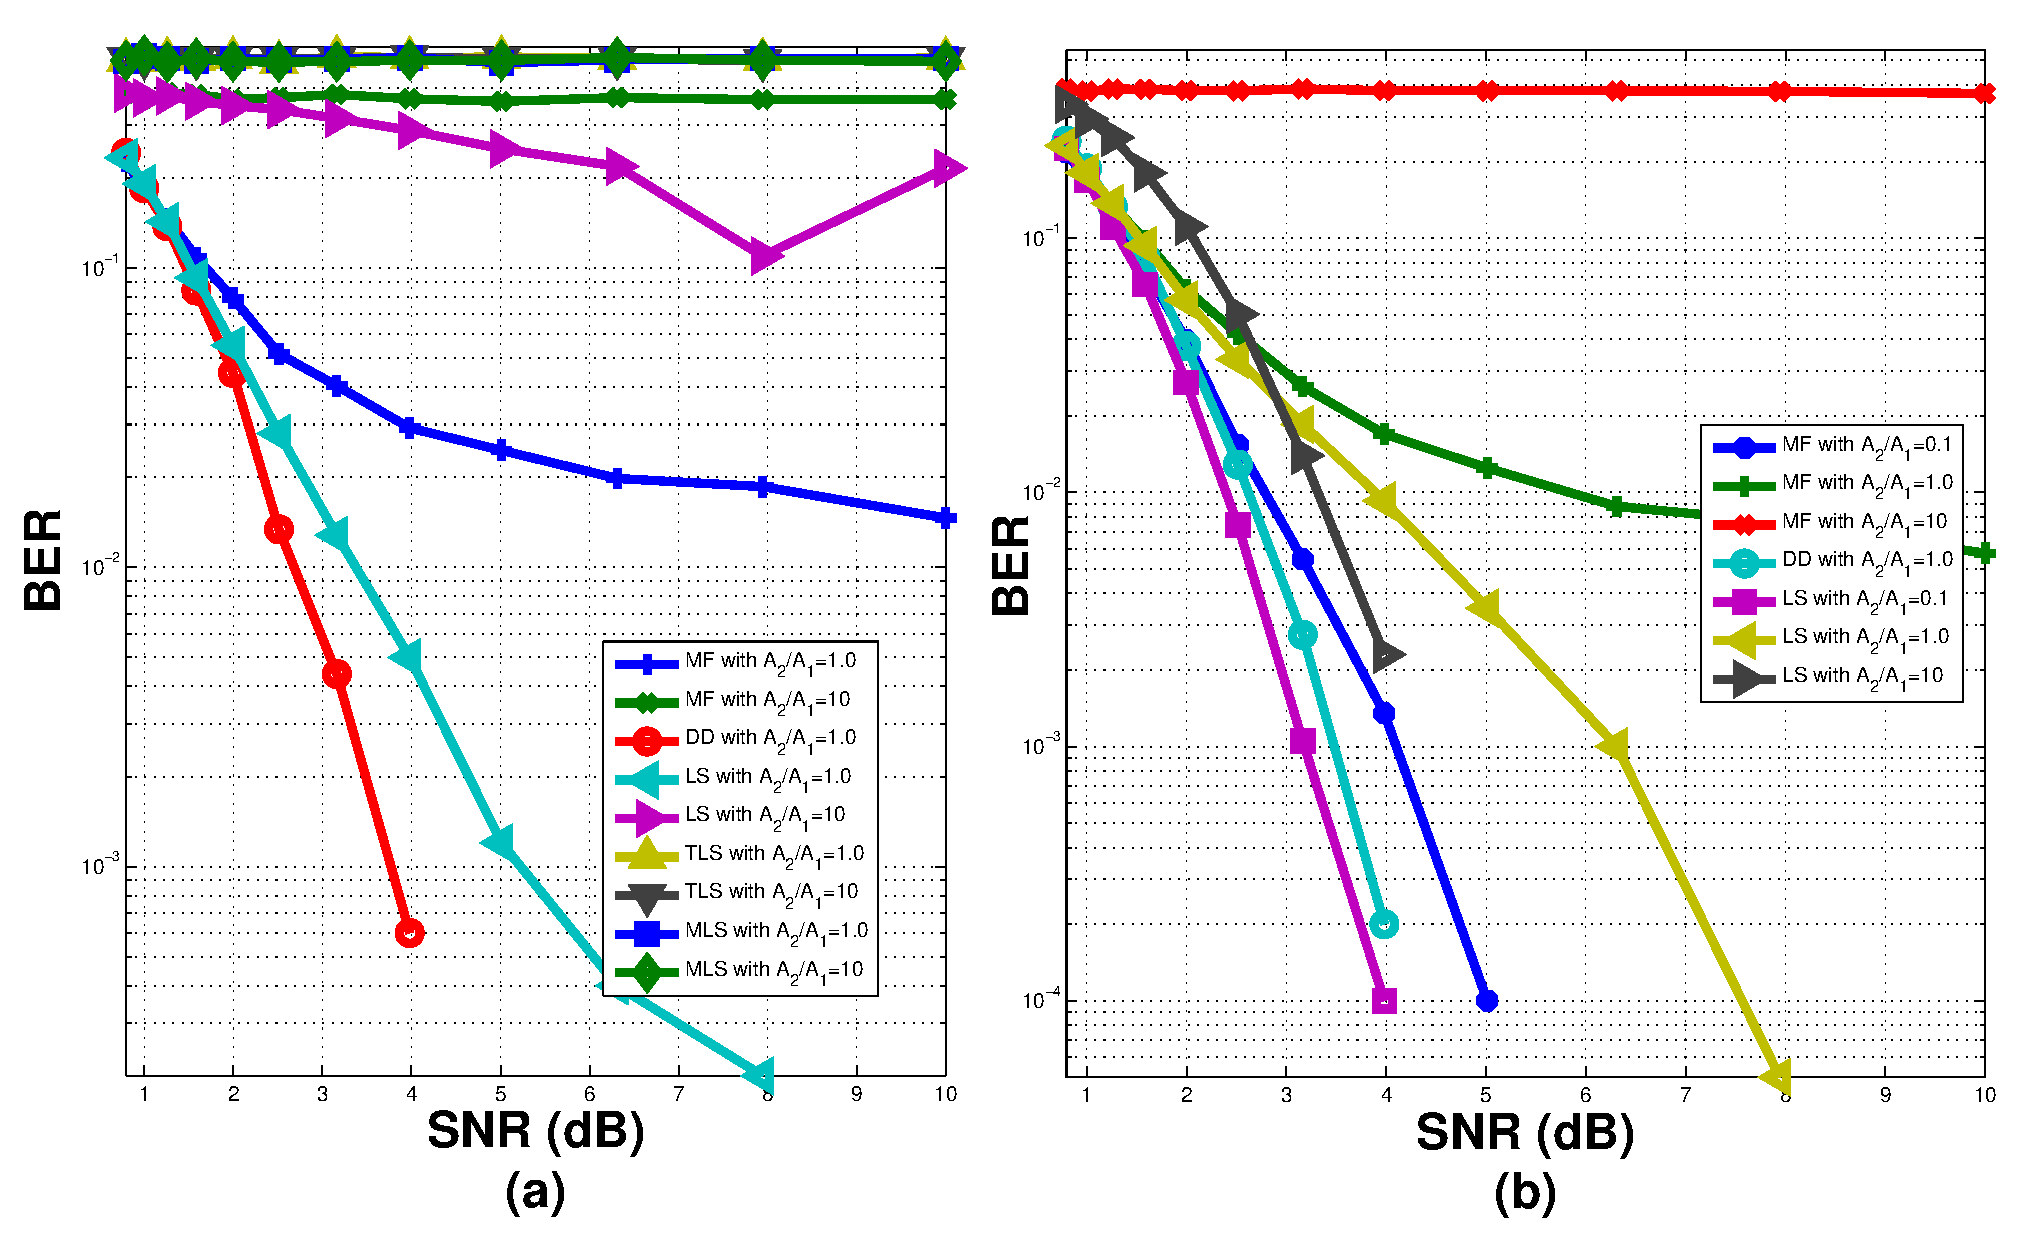
\includegraphics[width=3in]{BER_SNR_10_64.eps}
\caption{ (a) The performance of the proposed blind DF-ICs against
SNR, $M=12$. (b) The performance of the proposed blind LS
detector, $M=63$. } }\label{BER_SNR}
\end{figure}
\begin{figure} \center{
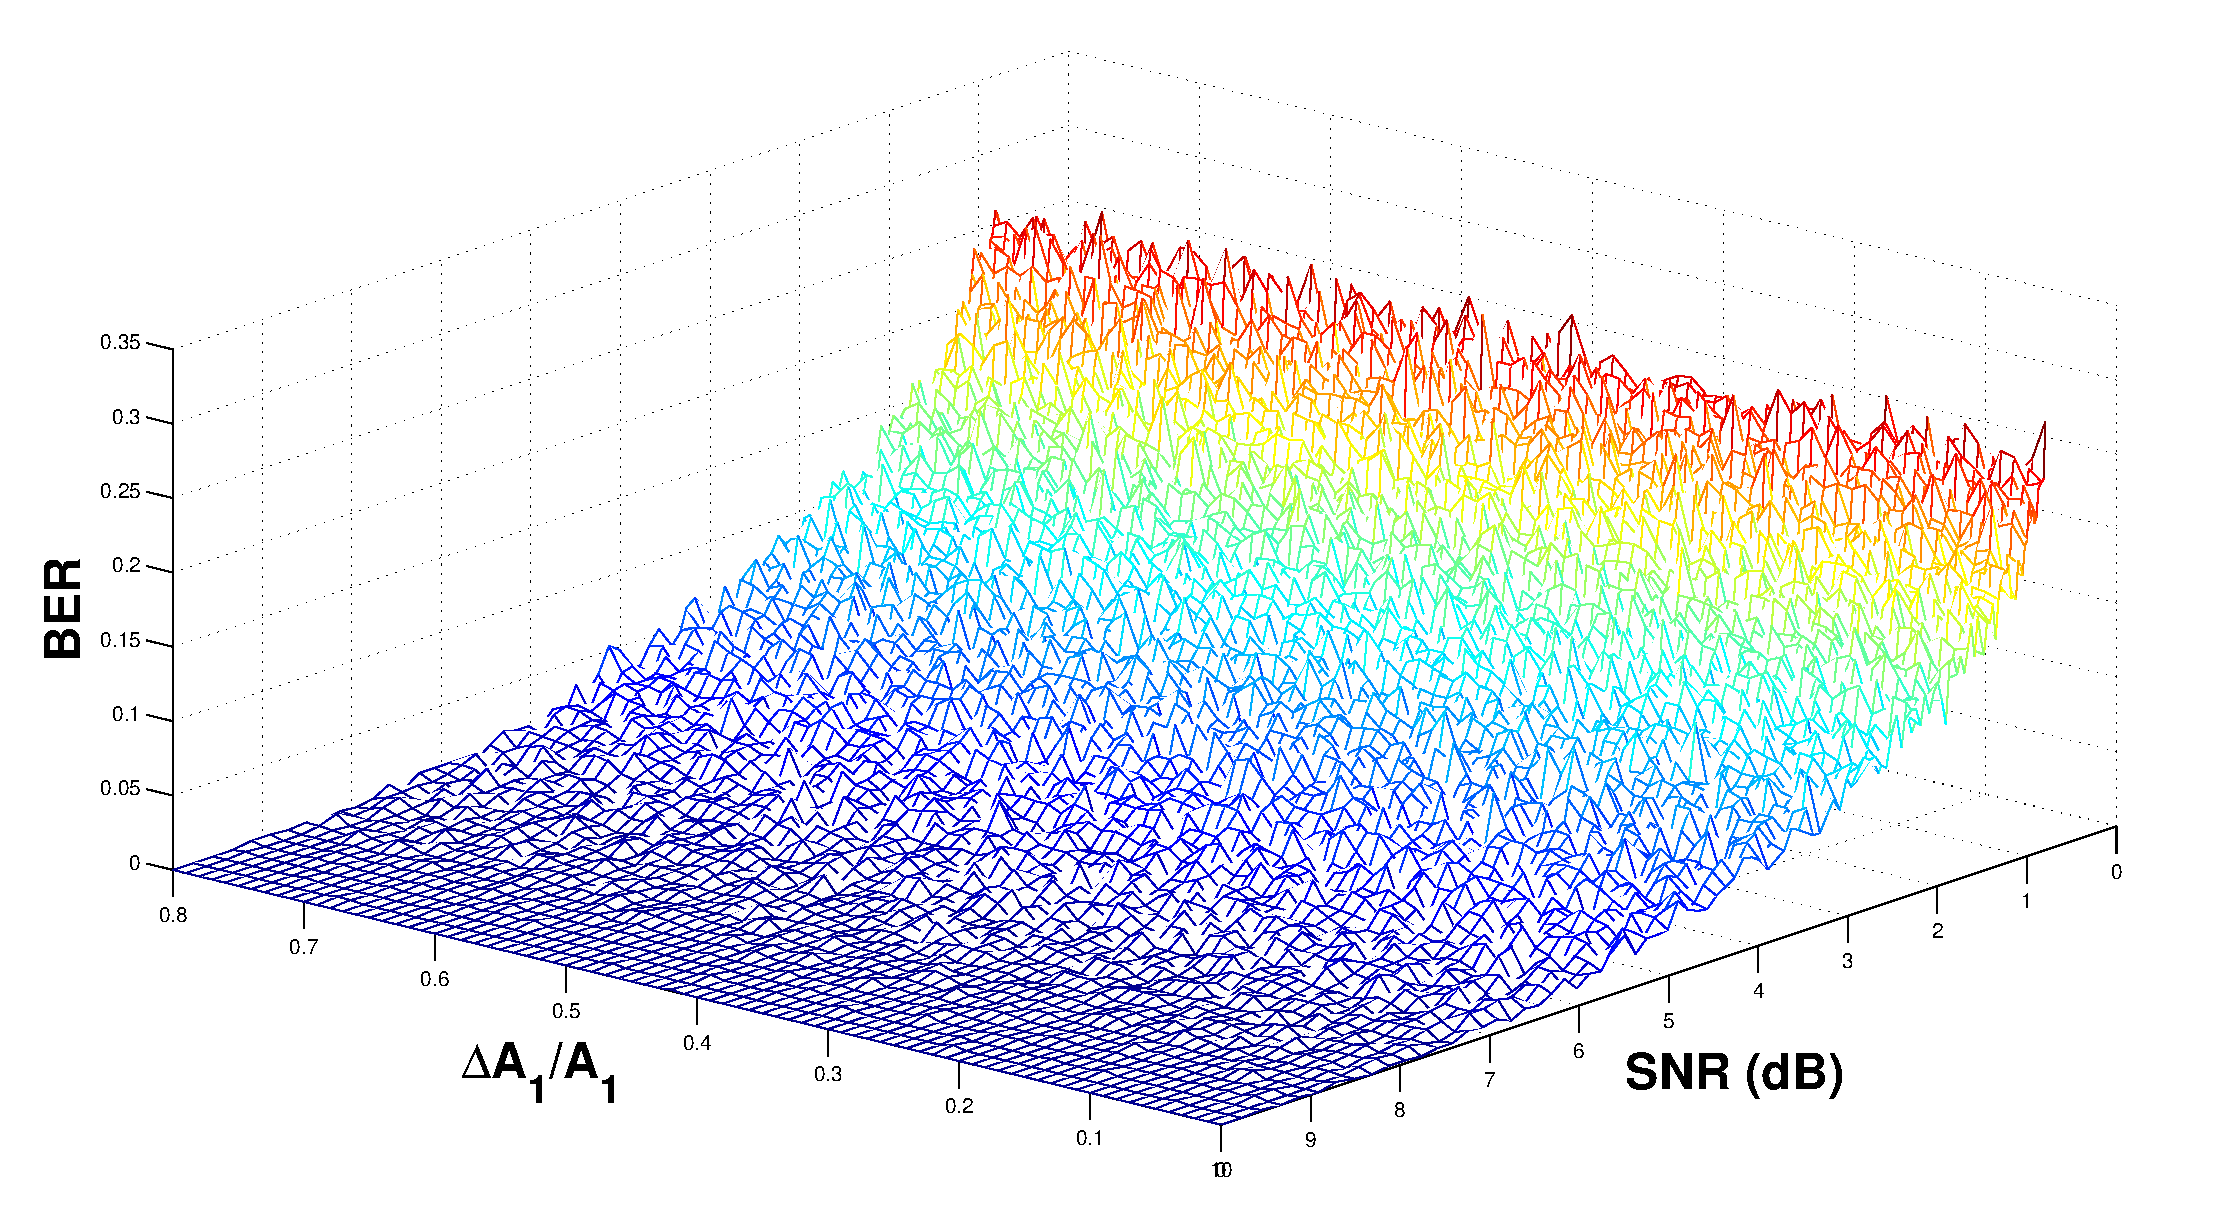
\includegraphics[width=2.5in]{BER_A_SNR_10_64_LSs.eps}
\caption{ The performance of the LS DF-IC against amplitude
estimation error ${\Delta}{A_1}/A_1$ and SNR, $M=63$.}
}\label{BER_A_SNR}
\end{figure}
\begin{figure}
\center{
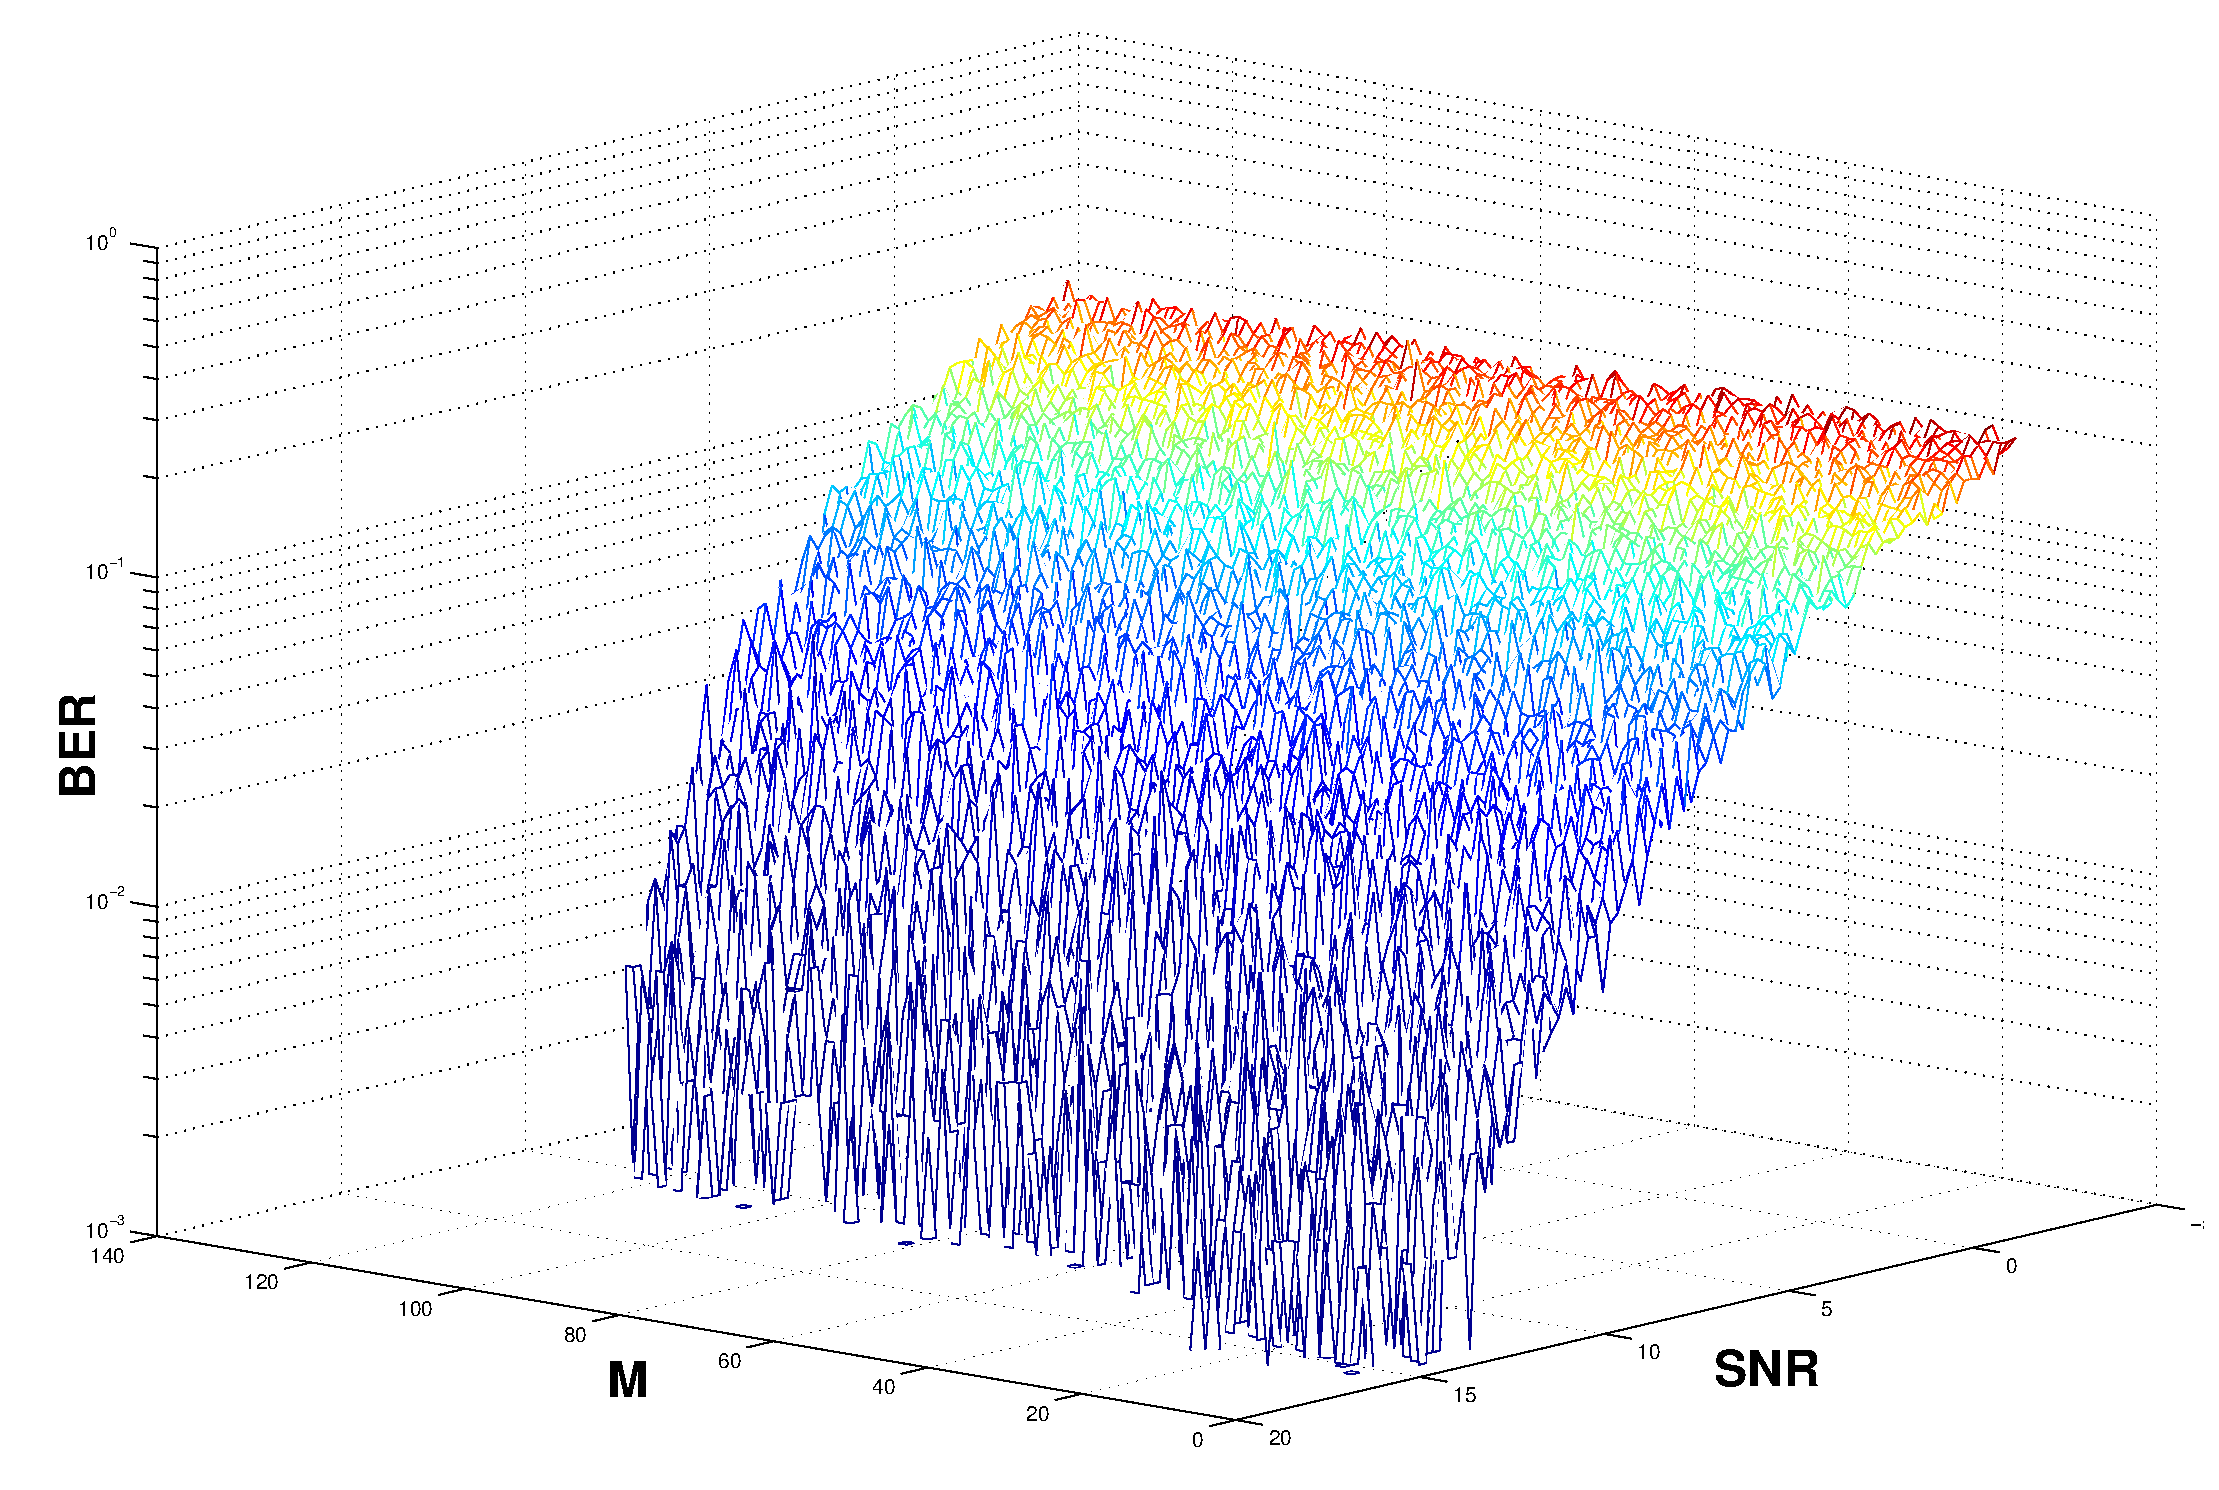
\includegraphics[width=2.5in]{BER_M_SNR_10_64_LSs.eps}
\caption{ The performance of the LS DF-IC against $M$ and SNR.}
}\label{BER_M_SNR}
\end{figure}
\section{Conclusions}
In this paper, we proposed a blind interference cancellation
framework as well as several implementations. They are simple and
direct and require a minimum amount of previous detected symbols.

\small\bibliographystyle{unsrt}
\bibliography{FastBDD,InterferenceCancellation}
\end{document}
